\documentclass{article}
\usepackage{amsmath, amssymb}
\usepackage{pgfplots}
\usepackage{tikz}
\usetikzlibrary{calc}

\begin{document}
\begin{figure}[h]
    \centering
    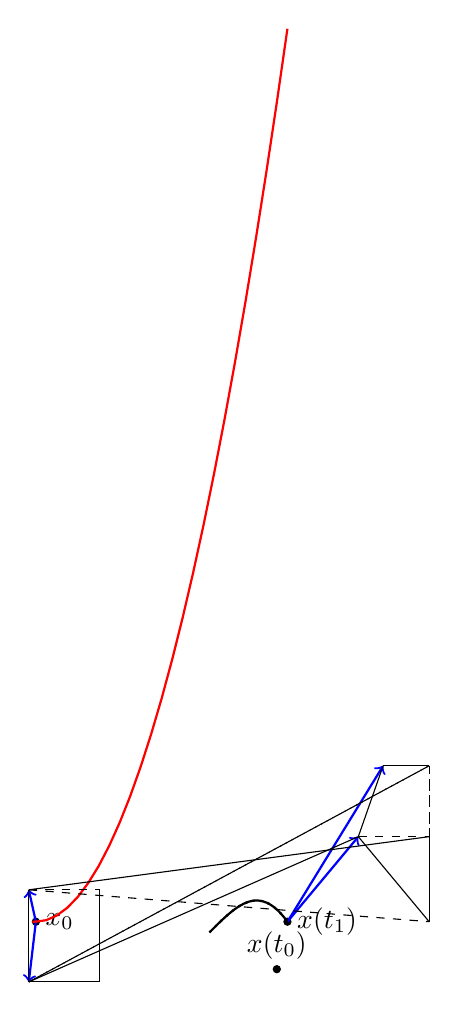
\begin{tikzpicture}[scale=0.9]
        \draw[fill=black] (2.35,-1.27) circle (0.05);
        \draw[fill=black] (-1.05, -0.6) circle (0.05);
        \draw[fill=black] (2.5,-0.6) circle (0.05);

        \node[above] at (2.35,-1.27) {$x(t_0)$};
        \node[right] at (-1.05, -0.6) {$x_0$};
        \node[right] at (2.5,-0.6) {$x(t_1)$};

        \draw[blue, thick, ->] (-1.05,-0.6) -- (-1.15, -1.45);
        \draw[blue, thick, ->] (-1.05,-0.6) -- (-1.15, -0.15);
        \draw[blue, thick, ->] (2.5,-0.6) -- (3.85, 1.6);
        \draw[blue, thick, ->] (2.5,-0.6) -- (3.5, 0.6);

        \draw[red, thick, domain=-1.1:-1.05] plot (\x,{(\x+1.1)*(\x+1.1)+(-0.6)});
        \draw[red, thick, domain=-1.05:2.5] plot (\x,{(\x+1.05)*(\x+1.05)+(-0.6)});

        \draw (-1.15, -1.45) -- (-1.15, -0.15);
        \draw[dashed] (-1.15, -0.15) -- (-0.15, -0.15);
        \draw (-1.15, -1.45) -- (-0.15, -1.45);
        \draw[dashed] (-0.15, -0.15) -- (-0.15, -1.45);
        \draw[dashed] (-0.15, -0.15) -- (-0.15, -0.6);
        \draw[dashed] (-0.15, -1.45) -- (-0.15, -0.6);

        \draw (3.85, 1.6) -- (3.5, 0.6);
        \draw[dashed] (3.5, 0.6) -- (4.5, 0.6);
        \draw (3.85, 1.6) -- (4.5, 1.6);
        \draw[dashed] (4.5, 0.6) -- (4.5, 1.6);
        \draw[dashed] (4.5, 0.6) -- (4.5, -0.6);
        \draw[dashed] (4.5, 1.6) -- (4.5, -0.6);

        \draw[dotted] (-1.15, -1.45) -- (4.5, 1.6);

        \draw (-1.15, -1.45) -- (4.5, 1.6);
        \draw (-1.15, -0.15) -- (4.5, 0.6);
        \draw[dashed] (-1.15, -1.45) -- (-0.15, -1.45);
        \draw[dashed] (-1.15, -0.15) -- (-0.15, -0.15);
        \draw (-0.15, -1.45) -- (-0.15, -0.6);
        \draw (-0.15, -0.15) -- (-0.15, -0.6);
        \draw (3.5, 0.6) -- (4.5, -0.6);
        \draw (4.5, 0.6) -- (4.5, -0.6);
        \draw[dashed] (4.5, 0.6) -- (4.5, -0.6);
        \draw[dashed] (4.5, -0.6) -- (4.5, -0.6);
        \draw (-1.15, -1.45) -- (3.5, 0.6);
        \draw[dashed] (-1.15, -0.15) -- (4.5, -0.6);

        \draw[thick, black] (1.4, -0.75) .. controls (1.8, -0.35) and (2.1, -0.05) .. (2.5, -0.6);
        \draw[thick, dashed, dotted] (1.4, -0.75) .. controls (1.8, -0.35) and (2.1, -0.05) .. (2.5, -0.6);
    \end{tikzpicture}
    \caption{Illustration of the preconditioning in~\protect\Cref{algo:preconditioning}. The point $x_{0}$ is an approximation of $x(t_{0})$. The blue line represents the predictor step, and the blue dotted line represents the corrector step to get an approximation $x_{1}$ of $x(t_{1})$. The line segment $s(t)$ connecting $x_{0}$ and $x_{1}$ is presented by the red line. The tilted interval box is centered at $s(t)$ at each $t\in[t_{0},t_{1}]$ with the same radius.}
    \label{fig:preconditioning}
\end{figure}
\end{document}